\begin{frame}
  {\texttt{\$ who}}

  \begin{columns}
    \begin{column}{0.48\textwidth}
      {\texttt{@f0rki}}
      \begin{itemize}
        \item CTF Player since 2010
      \end{itemize}
    \end{column}

    \begin{column}{0.48\textwidth}
      \texttt{@stefan2904}
      \begin{itemize}
        \item \ldots
      \end{itemize}
    \end{column}
  \end{columns}

\end{frame}


\begin{frame}{stuff we are gonna be talking about\ldots}
    \tableofcontents
\end{frame}


\section{Introduction to CTFs}

\begin{frame}[fragile]
  {Capture The Flag Competitions}

  \begin{itemize}
    \item Competitive hacking competitions
    \item Team-oriented
    \item The goal is to capture Flags:
      \begin{itemize}
        \item Like
          \verb+9447{ffmpeg_m0re_like_ffRCE_amirite}+ \\
          \verb+FAUST_VnSn2AwDAd1XxAAAAACjEEhYAjVLomA1+
        \item More flags \verb+==+ more points
      \end{itemize}
    \item Hack stuff and get flags
  \end{itemize}

\end{frame}

\begin{frame}
  {CTF Type: Jeopardy}

  \begin{center}
    %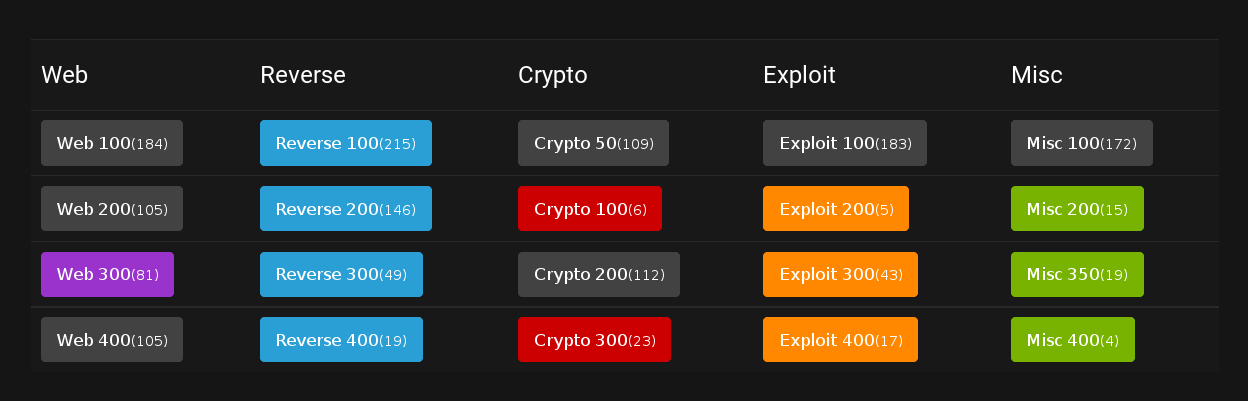
\includegraphics[width=\textwidth]{./images/dctf-challenges.png}
    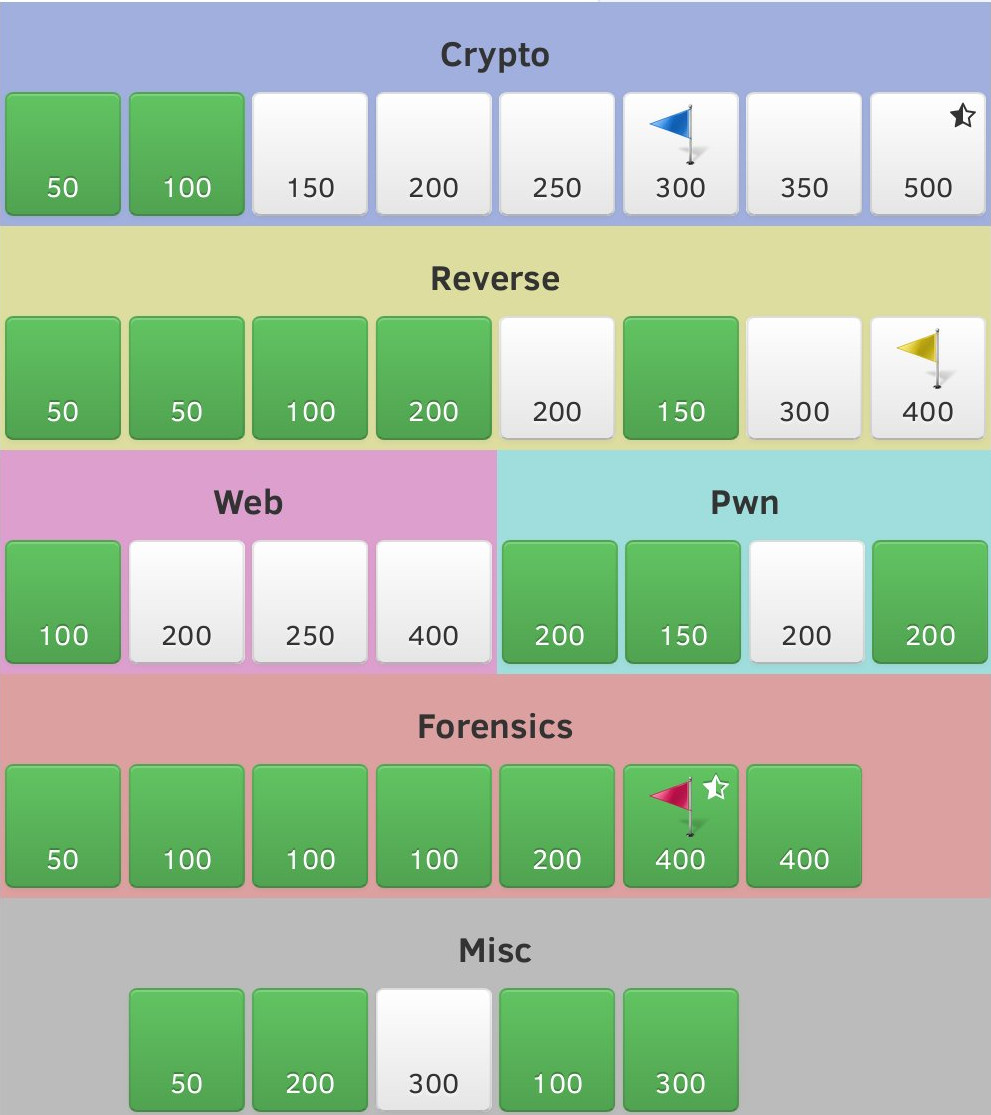
\includegraphics[height=0.8\textheight]{./images/sharifctf-challenges.jpg}
  \end{center}
\end{frame}

\begin{frame}
  {CTF Type: Attack-Defense}

  \begin{figure}[h]
    \centering
    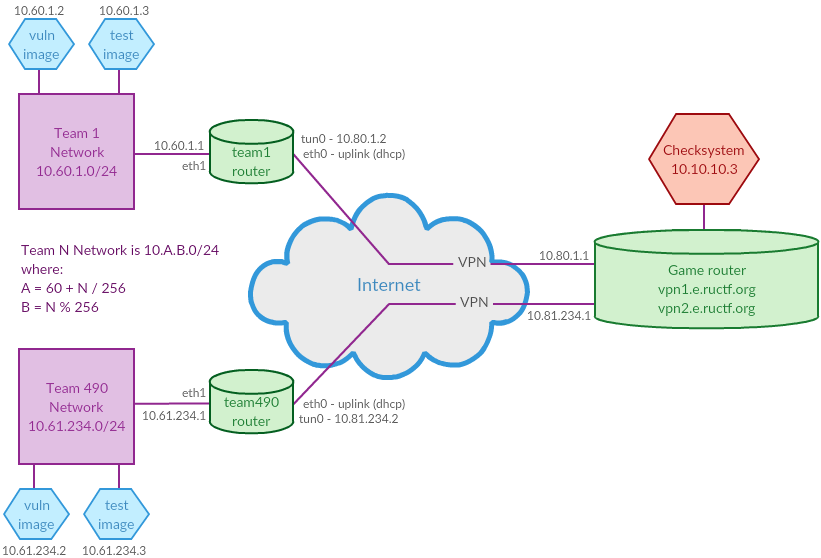
\includegraphics[width=0.9\textwidth]{./images/ructf-network.png}
    \caption{RUCTFe 2015 Network Schema (source:
      \href{https://ructf.org/e/2015/network.html}{RUCTF org}) }
  \end{figure}
\end{frame}
\begin{frame}
  {CTF Type: Attack-Defense}

  \begin{center}
    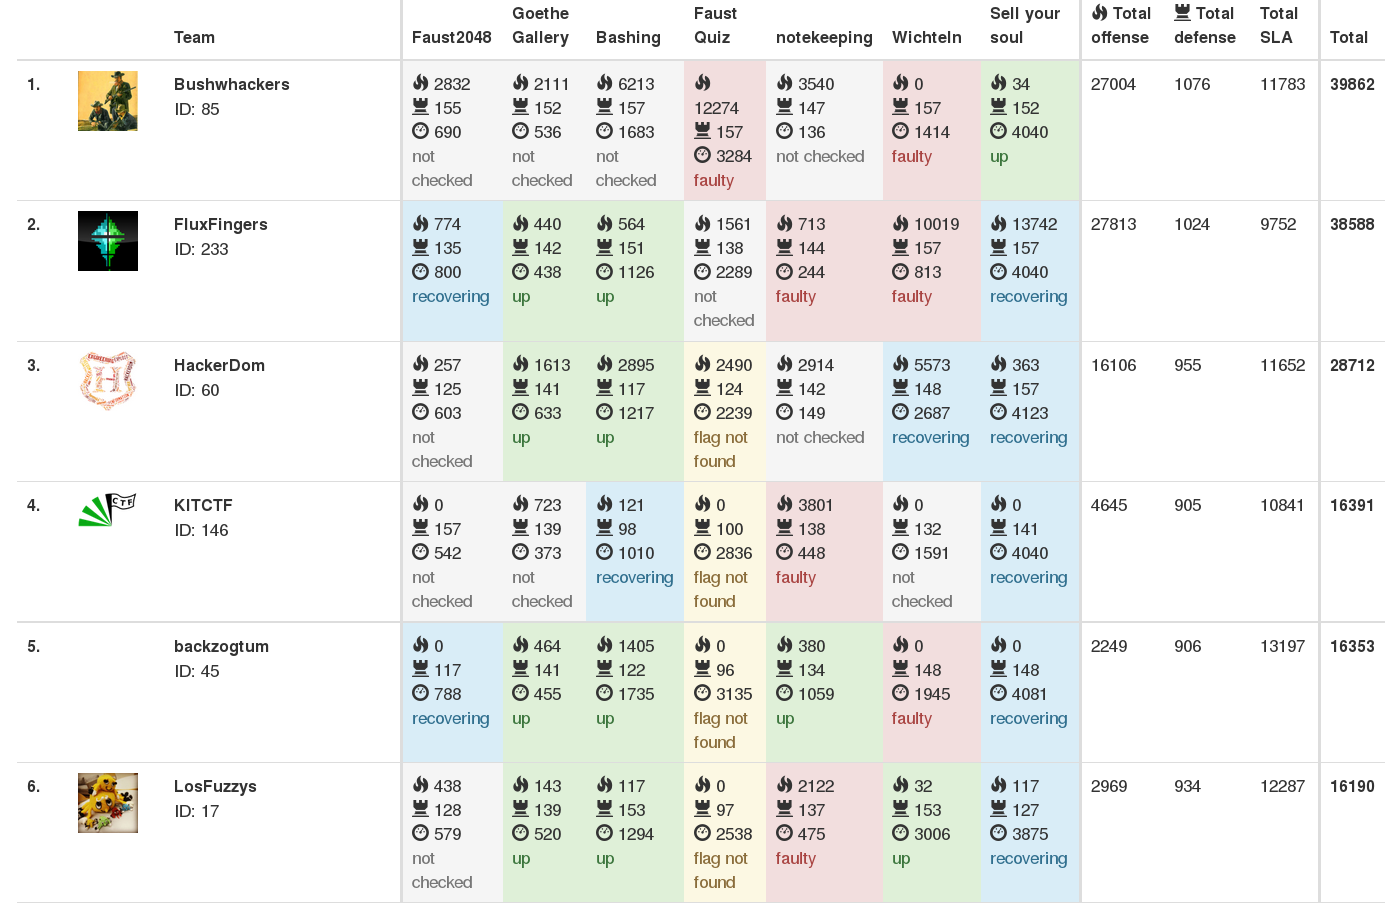
\includegraphics[width=\textwidth]{./images/faustctf-scoreboard.png}
  \end{center}

\end{frame}


\begin{frame}
  {Why CTFs?}

  \begin{itemize}
    \item \textbf{It's fun!}
    \item Gain experience in infosec
    \item Challenges modeled after real-world problems
  \end{itemize}
\end{frame}


\begin{frame}[allowframebreaks]
  {\texttt{LosFuzzys} CTF Team in Graz}
  {We Like Bugs!}

  \begin{figure}[H]
    \centering
    \includegraphics[height=0.7\textheight]{images/zippy/zippy_family2.jpg}
  \end{figure}

  \framebreak

  \begin{itemize}
    \item \url{http://hack.more.systems}
      \\ twitter: \href{https://twitter.com/LosFuzzys}{@LosFuzzys}
    \item A group of people interested in information security
    \item Primarily CS/SW/ICE Students from TUGraz
      \begin{itemize}
        \item But we welcome anyone interested and motivated :)
        \item and maybe even you ;)
      \end{itemize}
    \item Irregular Meet-ups
  \end{itemize}
\end{frame}

\begin{frame}
  {CTF Hackers Toolbox}

  \begin{itemize}
    \item Great diversity of challenges
    \item Some things turn up frequently
    \item Knowledge of technology necessary
    \item Experience helps a lot
  \end{itemize}

  \begin{itemize}
    \item Using the right tools is essential
      \begin{itemize}
        \item assuming you know how to use them\ldots
      \end{itemize}
  \end{itemize}

\end{frame}

\begin{frame}
  {Scripting is your best Friend}

  \begin{itemize}
    \item Python, Ruby, Bash etc.
    \item Be comfortable in one of those
  \end{itemize}

  \begin{center}
    
\includegraphics[height=0.5\textheight]{images/automatealltheexploits.jpg}
  \end{center}
\end{frame}


\begin{frame}
  {Command-Line-Fu is very helpful}

  \begin{itemize}
    \item Network stuff -- \texttt{nc, socat, dig, nmap}
    \item Query json files -- \texttt{jq}
    \item HTTP -- \texttt{curl}
  \end{itemize}

  \begin{itemize}
    \item Chain together to get your results!
  \end{itemize}
\end{frame}

% python requests - automated browsing

\begin{frame}[fragile]
  {Automated Browsing -- python-requests}

  \begin{lstlisting}[language=python]
import requests
s = requests.session()
URL = 'http://ctf.example.com'
r = s.post(URL + '/login',
           data={'user': 'fuzzy', 'pass': '1234'})
# session cookie automagically used here
print s.get(URL + '/vuln?x=\'or/**/1=1--x').text
  \end{lstlisting}
\end{frame}

% pwntools - implement parts of line-based network protocols

% pwntools - build exploits and pwn binaries

% radare2 - hex editor and disassembler

% gdb - pretty horrible
%peda
%https://github.com/cyrus-and/gdb-dashboard

% retdec decompiler

% pen & paper - never underestimate

% sagemath - crypto all the things

% apktool - disassemble and patch android apps



\begin{frame}
  {Learn to Improvise}

  \begin{itemize}
    \item Premature optimization* is the root of all evil!
      \begin{itemize}
        \item * also commenting code
        \item * also clean code
      \end{itemize}
    \item also everything above only \emph{during} CTFs
    \item If it works, \ldots it works!
    \item Code-reuse between different CTFs
  \end{itemize}

\end{frame}
